\chapter{Résultats et réponses à nos questions de recherche}


\section{}

L'éxécution s'est réalisé sur une machine équipée d'un processeur \textit{Intel Xeon E5-2620v4} avec 32 Gio de mémoire. Le temps nécessaire pour une analyse complète en x86\_64 avec \texttt{GCC 12.02} est de 4h07. Une analyse complète comprend la compilation de HACL*, la génération des fichiers de tests, la compilation desdits fichiers et l'analyse individuelle de chacun par Binsec. Nous avons ajouté un module pour synthétiser et générer des rapports d'analyse.\bigbreak

\begin{figure}[!ht]
  \centering
  \scalebox{0.65}{%
    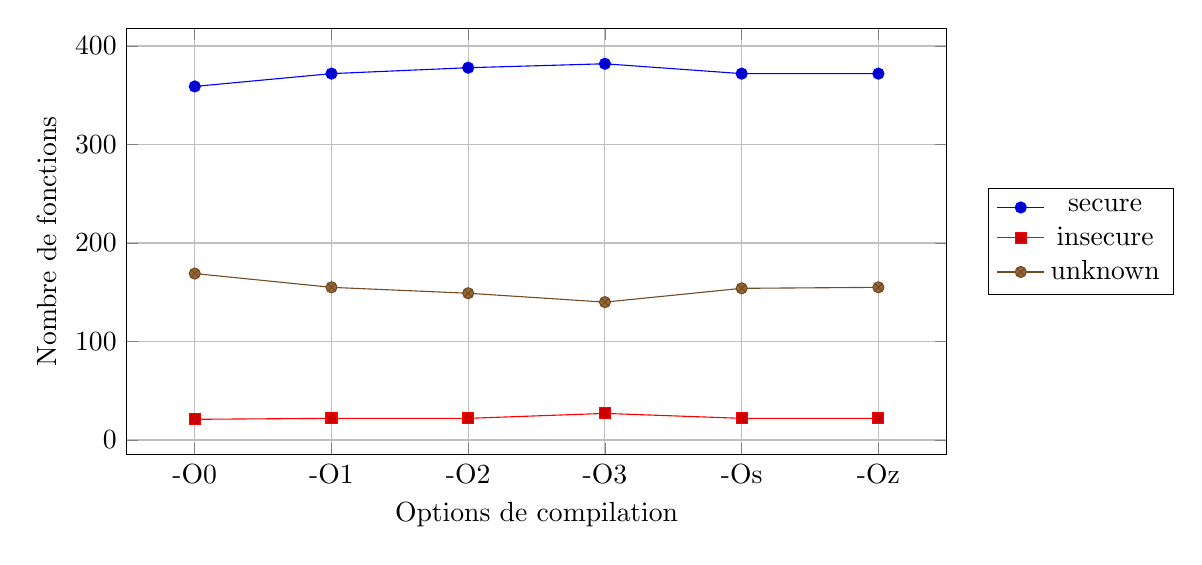
\begin{tikzpicture}
      \begin{axis}[
        xlabel={Options de compilation},
        ylabel={Nombre de fonctions},
        legend style={at={(0.5,-0.15)},anchor=north,legend columns=-1},
        grid=both,
        xtick={0,1,2,3,4,5},
        xticklabels={-O0, -O1, -O2, -O3, -Os, -Oz},
        width=12cm, height=7cm,
        legend style={at={(1.05,0.5)}, anchor=west},
        legend columns=1
      ]

        \addplot coordinates {(0,359) (1,372) (2,378) (3,382) (4,372) (5,372)};
        \addlegendentry{secure}

        \addplot coordinates {(0,21) (1,22) (2,22) (3,27) (4,22) (5,22)};
        \addlegendentry{insecure}

        \addplot coordinates {(0,169) (1,155) (2,149) (3,140) (4,154) (5,155)};
        \addlegendentry{unknown}

      \end{axis}
    \end{tikzpicture}%
  }
  \caption{Graphes des résultats d'Érysichthon en x86\_64}
  \label{fig:graphe_total}
\end{figure}


Les données détaillées peuvent être consultées en annexe \ref{tab:resultats_finaux}. En l'état, l'analyse rapporte entre 139 et 168 fichiers (en fonction des options de compilations, voir la figure \ref{fig:graphe_total}) dont l'analyse n'a pu se terminer. Il faudrait observer plus en détails ces fichiers pour connaître les causes précises de ces arrêts. Nous pouvons dans un premier temps faire une analyse haut niveau des raisons probables de ces intérruptions. \medbreak

\begin{figure}[!ht]
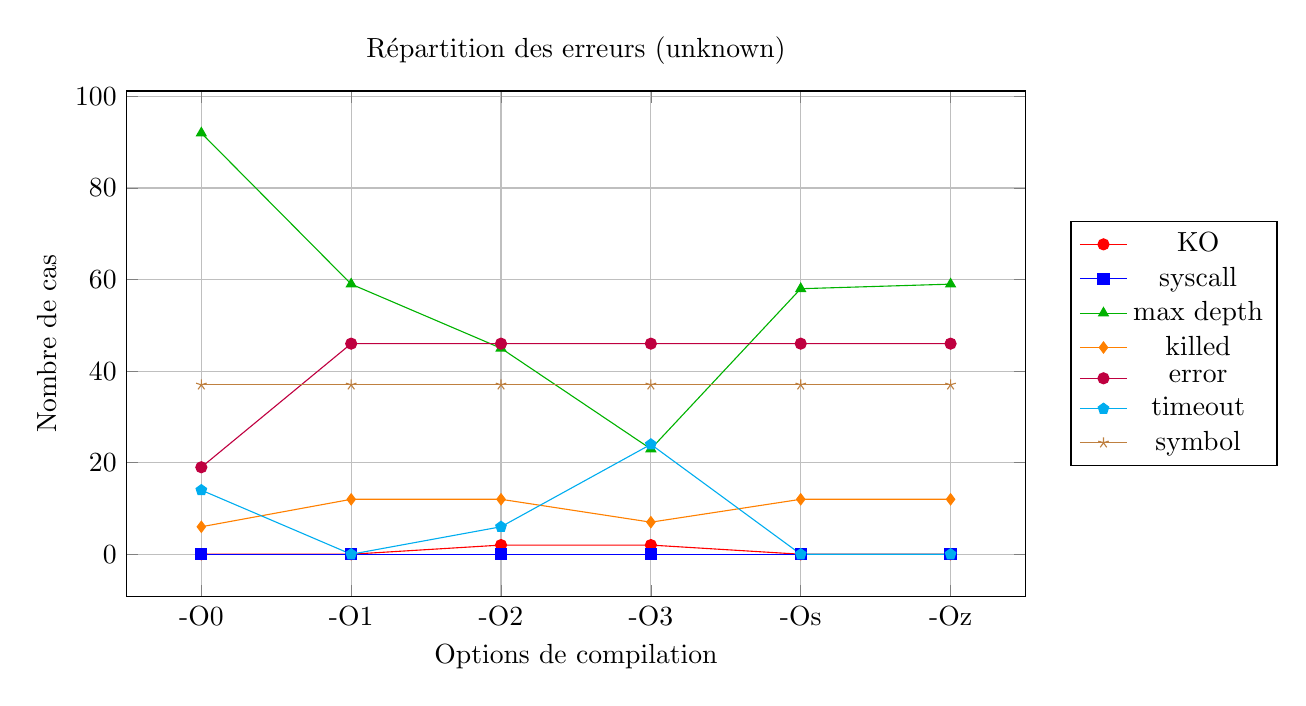
\begin{tikzpicture}
  \begin{axis}[
    title={Répartition des erreurs (unknown)},
    xlabel={Options de compilation},
    ylabel={Nombre de cas},
    grid=both,
    xtick={0,1,2,3,4,5},
    xticklabels={-O0, -O1, -O2, -O3, -Os, -Oz},
    width=13cm, height=8cm,
    legend style={at={(1.05,0.5)}, anchor=west}
  ]

    % KO
    \addplot[color=red, mark=*] coordinates {(0,0) (1,0) (2,2) (3,2) (4,0) (5,0)};
    \addlegendentry{KO}

    % syscall
    \addplot[color=blue, mark=square*] coordinates {(0,0) (1,0) (2,0) (3,0) (4,0) (5,0)};
    \addlegendentry{syscall}

    % max depth
    \addplot[color=green!70!black, mark=triangle*] coordinates {(0,92) (1,59) (2,45) (3,23) (4,58) (5,59)};
    \addlegendentry{max depth}

    % killed
    \addplot[color=orange, mark=diamond*] coordinates {(0,6) (1,12) (2,12) (3,7) (4,12) (5,12)};
    \addlegendentry{killed}

    % error
    \addplot[color=purple, mark=otimes*] coordinates {(0,19) (1,46) (2,46) (3,46) (4,46) (5,46)};
    \addlegendentry{error}

    % timeout
    \addplot[color=cyan, mark=pentagon*] coordinates {(0,14) (1,0) (2,6) (3,24) (4,0) (5,0)};
    \addlegendentry{timeout}

    % symbol
    \addplot[color=brown, mark=star] coordinates {(0,37) (1,37) (2,37) (3,37) (4,37) (5,37)};
    \addlegendentry{symbol}

  \end{axis}
\end{tikzpicture}
  \caption{Graphes détaillant les erreurs interrompant l'analyse Binsec}
  \label{fig:graphe_unknown}
\end{figure}

Le détail des valeurs est rapporté en annexe \ref{table:detail_unknown}.\smallbreak

On peut voir avec cette figure \ref{fig:graphe_unknown} que les erreurs sont dues à :
\begin{enumerate}
  \item[\texttt{max depth}] Arrêt par limitations du nombre d'instruction à analyser, cela permet de réduire la profondeur des branchement conditionnels à explorer et limiter le risque de parcours infini.
  \item[\texttt{timeout}] Comme le précédent, limitation par le temps. 
  \item[\texttt{killed}] Consommation excessive des ressources, processus interrompu. 
  \item[\texttt{error}] Instruction inconnue de Binsec, il a besoin que le script d'instruction soit corrigé.
  \item[\texttt{symbol}] Comme le précédent, mais peut-être que le fichier de test a besoin d'être modifié.
  \item[\texttt{KO}] Instruction inconnue de Binsec, il a besoin d'être amélioré. 
\end{enumerate}

Chaque erreur préconise un correctif à apporter à Érysichthon. Nous allons détailler les solutions qui nous sont apparus.

\subsection*{Correctifs à implémenter}

Pour résoudre la limitation \texttt{max depth}, nous utiliserons l'outil \texttt{perf}. Cela nous permet de déterminer le nombre d'instructions que contient le binaire. Identifier cette varaible nous permet d'exécuter la commande \ref{lst:commande_binsec} précisément.

Concernant l'erreur de type \texttt{timeout}, par défaut une exécution Binsec ne s'interrompt pas, nous avions ajouter ce garde-fou pour forcé l'arrêt de l'analyse de certaines fonctions qui s'étendaient dans le temps. Nos scripts Binsec ne présentant pas d'interruption dès la 
De même, avoir accès à une machine avec suffisement de mémoire vive nous permet de retirer la limitation \texttt{timeout}. Elle a été ajouté car l'analyse des fonctions \texttt{timeout}

\subsection*{Sécurité de HACL*}

Revenons sur les resultats présentés sur la figure \ref{fig:graphe_total} et ignorons les fonctions marquées \texttt{unknown}. Les fichiers non sécurisés sont les plus nombreux avec l'option \texttt{-O3} (27) et le moins avec l'option \texttt{-O0} (21). Nous retrouvons le détail des résultats en annexe \ref{tab:resultats_insecure}. Cette expérimentation confirme les travaux de \citeauthor{schneider2024breakingbadcompilersbreak}, en revanche, nous nous interrogeons quant à la réalité des fuites détectées par Érysichthon. Est-ce qu'une attaque peut réellement être réalisée ?\smallbreak
Nous analysons toute la bibliothèque HACL*, il est donc normal que certaines fonctions ne soient pas sécurisées car elle n'ont pas pour objectif de l'être. Peut importe les options de compilations que nou spouvons préciser. Ce sont des fonctions comme \texttt{Hacl\_P256\_\-vali\-date\_public\_key} ou \texttt{Hacl\_P256\_\-ecdsa\_\-verif\_p256\_sha384} qui effectuent des vérifications sur des données publiques. 

\begin{CitationBox}{est-ce que je peux finir sur ça ?}
  Actuellement dans la liste, aucune fonction indiquée non sécurisé ne demande une réimplémentation et peut être conservé dans la bibliothèque.
\end{CitationBox}


